% AA-30 | Iteracja XV
\chapter[Konstrukcje i wielokąty foremne]{Konstrukcje cyrklem i linijką oraz wielokąty foremne}
\label{aa:ch:constructibility}
\section{Algebraiczny opis konstrukcji}

W klasycznej geometrii wolno nam wykonywać wyłącznie skończenie
wiele rysunków prostych i okręgów. Trudność polega na wykazaniu,
że nawet bardzo sprytny wybór kolejnych przecięć nie pozwala
otrzymać wszystkich liczb rzeczywistych. Opiszemy algorytm
geometryczny za pomocą kolejnych rozszerzeń ciał stopnia
co najwyżej dwa. W ten sposób zagadnienia dotyczące
podwajania sześcianu, trysekcji kąta oraz wielokątów
foremnych sprowadzimy do precyzyjnych pytań algebraicznych.

Przyjmujemy ciało liczb rzeczywistych $\mathbb R$ jako już
dane; nie konstruujemy go w tym skrypcie. Punkty płaszczyzny
identyfikujemy z liczbami zespolonymi $x+iy$, gdzie
$x,y\in\mathbb R$ i $i^2=-1$.
\begin{definicja}\label{aa:def:constructible}
Niech $S\subset\mathbb C$ będzie skończonym zbiorem punktów
zawierającym $0$ i $1$. Punkt $z\in\mathbb C$ nazywamy
\emph{konstruowalnym z $S$ cyrklem i linijką}, jeśli istnieje
skończony ciąg zbiorów punktów
$S=S_0\subseteq S_1\subseteq\cdots\subseteq S_m$
taki, że $z\in S_m$, a każdy zbiór $S_j$ powstaje
z $S_{j-1}$ przez dołączenie jednego z \emph{izolowanych}
punktów przecięcia dwóch \emph{różnych} obiektów
następujących rodzajów:
\begin{enumerate}
\item prostych wyznaczonych przez dwa różne punkty
      z $S_{j-1}$;
\item okręgów o środku w punkcie z $S_{j-1}$
      i promieniu równym odległości dwóch punktów
      z $S_{j-1}$ (promień dodatni).
\end{enumerate}
Zaznaczenie izolowanego przecięcia jest dozwolone tylko,
jeżeli przecięcie istnieje. Nie wolno \emph{dowolnie} wybierać
punktu z dwóch pokrywających się prostych lub okręgów:
taki wybór nie stanowi skończonej konstrukcji.
Punkty już narysowane mogą być ponownie wykorzystywane;
wybór jednego z dwóch izolowanych przecięć jest dozwolony.
\end{definicja}
\begin{lemat}[Operacje arytmetyczne w konstrukcjach]
\label{aa:lem:constructibility-field-operations}
Jeżeli liczby rzeczywiste $a,b$ są konstruowalne z $\{0,1\}$,
to konstruowalne są także $a+b$, $a-b$ i $ab$.
Jeżeli ponadto $b\ne0$, konstruowalna jest liczba $a/b$.
Dla $a\ge0$ konstruowalna jest również liczba $\sqrt a\ge0$.
\end{lemat}
\begin{proof}
\textbf{Oś i współrzędne.}
Prosta przez $0,1$ jest osią rzeczywistą. Okrąg
o środku $0$ i promieniu $1$ przecina tę oś
w punktach $1$ i $-1$. Dwa okręgi o promieniu $2$,
równym długości już skonstruowanego odcinka $[-1,1]$,
których środkami są
$1$ i $-1$, przecinają się w dwóch punktach
leżących po przeciwnych stronach osi. Prosta przez
te przecięcia jest symetralną odcinka $[-1,1]$,
ponieważ oba punkty są jednakowo odległe od $1$
i $-1$. Jest to oś prostopadła do osi rzeczywistej
w punkcie $0$. Jej przecięcie z okręgiem jednostkowym
pozwala wybrać punkt $i=(0,1)$.

Ten sam algorytm zastosowany do dwóch punktów
na dowolnej skonstruowanej prostej daje symetralną
ich odcinka. Aby skonstruować prostopadłą przez
punkt $P$ należący do prostej, zaznaczamy dwa
punkty na tej prostej jednakowo odległe od $P$
i konstruujemy ich symetralną. Dla punktu poza
prostą najpierw konstruujemy jego rzut prostopadły
na prostą: okrąg o środku w $P$ przecina prostą
w dwóch punktach (wybieramy dostatecznie duży
konstruowalny promień, np. kolejne podwojenia długości
ustalonego odcinka aż do przekroczenia odległości
$P$ od prostej), a ich symetralna
przechodzi przez $P$. Konstruując następną
prostopadłą do uzyskanej, otrzymujemy równoległą
do pierwszej prostej przechodzącą przez zadany punkt.
Przenoszenie odcinków na osie odbywa się za pomocą
okręgów o odpowiednich promieniach; wybór jednego
z dwóch przecięć ustala znak współrzędnej.
Przykładanie kolejnych odcinków zorientowanych
na tej samej osi daje dodawanie i odejmowanie.

\textbf{Mnożenie.}
Współrzędne $1$, $a$ i $b$ możemy zaznaczyć
na osi rzeczywistej; korzystając z prostopadłych,
umieszczamy także punkt $(0,b)$. Rysujemy prostą
przez punkty $(1,0)$ oraz $(0,b)$, o równaniu
$y=b(1-x)$. Prosta przez $(a,0)$ równoległa
do niej ma równanie $y=b(a-x)$ i przecina
oś pionową w $(0,ab)$. Aby przenieść tę podpisaną
współrzędną na oś poziomą,
konstruujemy prostą $y=x$ przez $0$ i $(1,1)$; ten drugi
punkt jest przecięciem pionowej przez $1$ i poziomej przez $i$.
Odbicie $(0,ab)$ względem prostej $y=x$ jest konstrukcją
cyrklem i linijką (przez rzut prostopadły i odłożenie
tej samej odległości po przeciwnej stronie prostej)
i daje punkt $(ab,0)$.

\textbf{Dzielenie.}
Tym samym twierdzeniem o podobieństwie trójkątów,
stosując prostą o nachyleniu zadanym przez
punkty $(b,0)$, $(0,a)$ i prostą równoległą
przechodzącą przez $(1,0)$, otrzymujemy
na osi pionowej współrzędną $a/b$.
Rzeczywiście nachylenie pierwszej prostej wynosi
$-a/b$, więc równoległa przechodząca przez $(1,0)$
ma punkt przecięcia z osią pionową $(0,a/b)$.
Założenie $b\ne0$ gwarantuje, że użyty odcinek
na osi poziomej jest niezerowy.

\textbf{Pierwiastek kwadratowy.}
Dla $a>0$ kreślimy okrąg o średnicy
$[0,1+a]$ na osi rzeczywistej, a następnie
prostą prostopadłą do osi w punkcie $1$.
Jeśli $(1,y)$ należy do okręgu, to jego równanie daje
\[
 \left(1-\frac{1+a}{2}\right)^2+y^2
 =\left(\frac{1+a}{2}\right)^2,
 \qquad y^2=a.
\]
Wybieramy przecięcie z $y>0$, otrzymując $\sqrt a$.
Dla $a=0$ pierwiastek wynosi $0$ i jest już dany.
W każdej konstrukcji użyto tylko dozwolonych
izolowanych przecięć prostych i okręgów.
\end{proof}

\begin{twierdzenie}[Kryterium wieży kwadratowej]\label{aa:tw:constructibility-tower}
Dla każdego $z=x+iy\in\mathbb C$, gdzie $x,y\in\mathbb R$,
następujące warunki są równoważne:
\begin{enumerate}
\item punkt $z$ jest konstruowalny z $\{0,1\}$;
\item istnieje liczba całkowita $r\ge0$ i wieża podciał
$\mathbb Q=K_0\subseteq K_1\subseteq\cdots\subseteq K_r
\subseteq\mathbb R$ taka, że
$[K_j:K_{j-1}]\le2$ dla każdego $1\le j\le r$
oraz $x,y\in K_r$.
\end{enumerate}
\end{twierdzenie}
\begin{proof}
\textbf{Od konstrukcji do wieży.}
Współrzędne punktów początkowych $0,1$ należą do
$K_0=\mathbb Q$. Załóżmy, że wszystkie otrzymane
punkty mają współrzędne w ustalonym podciele
$K\subseteq\mathbb R$. Prosta przez dwa różne takie
punkty ma równanie $Ax+By=C$, gdzie $A,B,C\in K$
oraz $(A,B)\ne(0,0)$. Okrąg o środku $(a,b)$
i promieniu równym odległości znanych punktów
ma równanie $(x-a)^2+(y-b)^2=R$, gdzie
$a,b,R\in K$, $R>0$.

Dwie różne proste mają co najwyżej jeden punkt
przecięcia. Jeżeli go mają, układ dwóch równań
liniowych ma niezerowy wyznacznik, więc obie
współrzędne punktu należą do $K$.
W przypadku przecięcia prostej z okręgiem
parametryzujemy prostą jako
$(x,y)=(x_0,y_0)+t(u,v)$, gdzie
$x_0,y_0,u,v\in K$ i $(u,v)\ne(0,0)$.
Po podstawieniu do równania okręgu dostajemy
$At^2+Bt+C=0$ z $A=u^2+v^2>0$ i
$A,B,C\in K$. Każdy parametr $t$ wybranego
punktu przecięcia ma stopień co najwyżej $2$
nad $K$; obie współrzędne należą do tego samego
ciała $K(t)$.

Jeżeli przecinamy dwa okręgi o różnych środkach,
to po odjęciu ich równań otrzymujemy równanie
prostej o niezerowym wektorze współczynników
w $K^2$. Punkty przecięcia obu okręgów
należą również do tej prostej, więc wracamy
do poprzedniego przypadku. Okręgi współśrodkowe
i różne nie mają punktów wspólnych; okręgi
pokrywające się nie dają dozwolonego izolowanego
przecięcia. W każdym kroku współrzędne nowego
punktu należą zatem do jednego rzeczywistego
rozszerzenia stopnia $1$ lub $2$. Dołączając te
rozszerzenia kolejno, otrzymujemy wymaganą wieżę.

\textbf{Od wieży do konstrukcji.}
Indukujemy po liczbie poziomów wieży. Każda liczba
w $K_0=\mathbb Q$ jest konstruowalna dzięki
Lematowi~\ref{aa:lem:constructibility-field-operations}.
Przypuśćmy, że skonstruowaliśmy wszystkie liczby
$K_{j-1}$. Jeśli $K_j=K_{j-1}$, niczego nie
trzeba dodawać. W przeciwnym razie rozszerzenie
$K_j/K_{j-1}$ jest kwadratowe, więc istnieje
$u\in K_j$ takie, że $K_j=K_{j-1}(u)$, a jego
wielomian minimalny ma postać
$T^2+bT+c$ dla $b,c\in K_{j-1}$.
Ponieważ $u\in\mathbb R$, wyróżnik
$d=b^2-4c=(2u+b)^2$ jest nieujemny.
Z lematu potrafimy skonstruować
$\sqrt d$ i obie wartości $(-b\pm\sqrt d)/2$,
w tym wybrane $u$. Każdy element $K_j$ ma postać
$a+bu$ dla pewnych $a,b\in K_{j-1}$,
więc jest konstruowalny z indukcji i lematu.
Po $r$ krokach konstruowalne są $x$ i $y$,
a przecięcie prostej pionowej przez $(x,0)$
z poziomą przez $(0,y)$ daje punkt $(x,y)$.
\end{proof}

\begin{wniosek}[Przeszkoda stopnia]\label{aa:cor:constructibility-degree}
Jeżeli liczba rzeczywista $a$ jest konstruowalna z $\{0,1\}$, to stopień $[\mathbb Q(a):\mathbb Q]$ jest potęgą liczby $2$.
\end{wniosek}
\begin{proof}
Z Twierdzenia~\ref{aa:tw:constructibility-tower} istnieje
wieża kwadratowa zawierająca $a$. Prawo wieży daje
$[K_r:\mathbb Q]=\prod_{j=1}^r[K_j:K_{j-1}]=2^m$
dla pewnego $m\ge0$: każdy czynnik jest równy $1$ lub $2$.
Ponieważ $\mathbb Q\subseteq\mathbb Q(a)\subseteq K_r$,
ponowne zastosowanie prawa wieży daje
$[K_r:\mathbb Q]=[K_r:\mathbb Q(a)]\,[\mathbb Q(a):\mathbb Q]$.
Dodatni dzielnik potęgi $2$ również jest potęgą $2$.
\end{proof}
\begin{lemat}[Domknięcie normalne wieży kwadratowej]
\label{aa:lem:quadratic-tower-normal-closure}
Niech $K$ będzie ciałem charakterystyki różnej od $2$ i
$K=K_0\subseteq K_1\subseteq\cdots\subseteq K_r$
skończoną wieżą rozszerzeń, w której
$[K_j:K_{j-1}]\le2$ dla każdego $j$. Wówczas
normalne domknięcie $K_r/K$ jest skończonym rozszerzeniem
Galois, którego grupa Galois ma rząd będący potęgą $2$.
\end{lemat}
\begin{proof}
Postępujemy indukcyjnie po liczbie poziomów wieży.
Dla $r=0$ domknięcie normalne jest równe $K$.
Przypuśćmy, że istnieje skończone rozszerzenie Galois
$E/K$ zawierające $K_{r-1}$ i takie, że
$\operatorname{Gal}(E/K)$ jest $2$-grupą.
Ponieważ charakterystyka jest różna od $2$, każde
właściwe rozszerzenie kwadratowe ma postać
$K_r=K_{r-1}(\sqrt d)$ dla pewnego
$d\in K_{r-1}^{\times}$. Gdy stopień jest równy $1$,
wystarczy przyjąć $E$ bez zmian.
Niech $G=\operatorname{Gal}(E/K)$ i niech
\[
 F=E\bigl(\sqrt{\sigma(d)}:\sigma\in G\bigr)
\]
we wspólnym domknięciu algebraicznym. Każde kolejne
dołączenie pierwiastka kwadratowego zwiększa stopień
co najwyżej dwukrotnie, a $F/E$ jest rozdzielcze i normalne,
ponieważ jest ciałem rozkładu rodziny wielomianów
$T^2-\sigma(d)$. Zatem $\operatorname{Gal}(F/E)$
jest $2$-grupą (jego rząd równa się $[F:E]$).
Ponadto każdy $K$-automorfizm domknięcia algebraicznego
zachowuje $E$ i permutuje wielomiany $T^2-\sigma(d)$,
więc zachowuje ich ciało rozkładu $F$. Stąd $F/K$ jest
normalne. Jest też rozdzielcze, a więc Galois.
Restrykcja automorfizmów daje dokładny ciąg
\[
1\longrightarrow\operatorname{Gal}(F/E)
\longrightarrow\operatorname{Gal}(F/K)
\longrightarrow\operatorname{Gal}(E/K)
\longrightarrow1,
\]
co wynika z normalności obu rozszerzeń. Rząd grupy
środkowej jest iloczynem rzędów skrajnych, czyli potęgą $2$.
Ponieważ $K_r\subseteq F$, jego domknięcie normalne nad $K$
zawiera się w $F$ i ma grupę Galois będącą ilorazem
podgrupy odpowiedniej grupy Galois $F/K$, a więc także
$2$-grupą. To kończy indukcję.
\end{proof}

\begin{uwaga}[Odwrotność jest fałszywa]\label{aa:uw:constructibility-degree-not-sufficient}
Sam fakt, że liczba algebraiczna ma stopień równy potędze $2$,
\emph{nie} zapewnia jej konstruowalności. W celu podania
sprawdzalnego przykładu rozważmy
$f(X)=X^4-X-1\in\mathbb Q[X]$.

\textbf{Nierozkładalność.}
Modulo $2$ otrzymujemy $\overline f=X^4+X+1$.
Nie ma on pierwiastka w $\mathbb F_2$, bo wartości
dla $0$ i $1$ są równe $1$. Jedynym monicznym
nierozkładalnym wielomianem kwadratowym nad
$\mathbb F_2$ jest $q=X^2+X+1$.
W ilorazie $\mathbb F_2[X]/(q)$ mamy $X^2=X+1$
i $X^4=X$, skąd $\overline f\equiv1\pmod q$.
Nie istnieje więc podział $\overline f$ na czynniki
stopni $1+3$ ani $2+2$, co dowodzi nierozkładalności
$\overline f$, a następnie $f$ nad $\mathbb Q$.
Każdy pierwiastek $f$ ma zatem stopień $4$ nad $\mathbb Q$.

\textbf{Działanie Galois na trzech podziałach.}
Niech $a,b,c,d$ oznaczają cztery różne pierwiastki
$f$ w ciele rozkładu $L$. Są one różne,
ponieważ $f$ jest nierozkładalny nad $\mathbb Q$,
a jego pochodna $f'=4X^3-1$ jest niezerowa i ma stopień
mniejszy niż $f$, wielomiany $f$ i $f'$ są względnie
pierwsze. W charakterystyce $0$ oznacza to, że $f$
jest rozdzielczy.
Definiujemy trzy liczby
\[
 u_1=ab+cd,\qquad u_2=ac+bd,\qquad u_3=ad+bc.
\]
Każda permutacja pierwiastków permutuje te liczby:
reprezentują one trzy podziały zbioru czterech
indeksów na dwie nieuporządkowane pary.
Oznaczmy przez $e_j$ elementarną sumę iloczynów
$j$ różnych elementów zbioru $\{a,b,c,d\}$.
Porównując współczynniki w tożsamości
\[
\prod_{t\in\{a,b,c,d\}}(X-t)
=X^4-e_1X^3+e_2X^2-e_3X+e_4=X^4-X-1,
\]
otrzymujemy $e_1=e_2=0$, $e_3=1$, $e_4=-1$.
Bezpośrednie rozwinięcie trzech iloczynów daje
\[
 u_1+u_2+u_3=e_2=0,
\]
\[
 u_1u_2+u_1u_3+u_2u_3=e_1e_3-4e_4=4,
\]
\[
 u_1u_2u_3=e_3^2+e_1^2e_4-4e_2e_4=1.
\]
Stąd $u_1,u_2,u_3$ są pierwiastkami wielomianu
$R(Y)=Y^3+4Y-1$. Ponieważ jedynymi możliwymi
pierwiastkami wymiernymi monicznego wielomianu
$R$ są $1$ i $-1$, a $R(1)=4$ i $R(-1)=-6$,
$R$ jest nierozkładalny nad $\mathbb Q$.
Jest też rozdzielczy: jego pochodna formalna
$R'=3Y^2+4$ jest niezerowym wielomianem stopnia $2$,
a $R$ jest nierozkładalny stopnia $3$ nad ciałem
charakterystyki $0$. Zatem $R$ i $R'$ nie mają
wspólnego nietrywialnego dzielnika, a w konsekwencji
$R$ nie ma pierwiastka wielokrotnego.
Można również sprawdzić, że wyróżnik $R$ wynosi $-283$.
Jego grupa Galois działa zatem przechodnio na
$u_1,u_2,u_3$. W rezultacie grupa
$G=\operatorname{Gal}(L/\mathbb Q)$ ma rząd
podzielny przez $3$ (Twierdzenie~\ref{aa:tw:orbita-stabilizator}).
Działanie $G$ na czterech pierwiastkach $f$
również jest przechodnie, więc $4$ dzieli $|G|$.
Ponieważ $G\subseteq S_4$, jej rząd dzieli $24$;
jedynymi możliwościami są $|G|=12$ lub $|G|=24$.

\textbf{Wykluczenie rzędu $12$.}
Wielomian $f$ ma dokładnie dwa pierwiastki rzeczywiste:
pochodna $f'=4X^3-1$ ma jedno rzeczywiste miejsce
zerowe $x_0>0$. Funkcja $f$ jest ściśle malejąca
na $(-\infty,x_0)$, rosnąca na $(x_0,\infty)$,
a $f(0)=-1$ i $f(x)\to+\infty$ dla $x\to\pm\infty$.
Pozostałe dwa pierwiastki tworzą parę sprzężoną
zespolenie. Sprzężenie zespolone jest automorfizmem
$L/\mathbb Q$, który ustala dwa rzeczywiste
pierwiastki i zamienia dwa nierzeczywiste, czyli
jest transpozycją w $G$.
Gdyby $|G|=12$, $G$ byłaby podgrupą indeksu $2$
w $S_4$, a więc normalną. Wszystkie transpozycje
w $S_4$ są sprzężone i generują $S_4$.
Niezerowy homomorfizm $S_4\to C_2$ musi zatem
wysyłać każdą transpozycję na niezerowy element,
więc jego jądro jest dokładnie $A_4$.
Taka podgrupa nie może zawierać transpozycji.
Dlatego $|G|=24$ i $G=S_4$.

\textbf{Dodatkowa kontrola arytmetyczna.}
Przy redukcji $f$ modulo $7$ otrzymujemy rozkład
\[
 X^4-X-1\equiv (X-3)(X^3+3X^2+2X-2)\pmod 7.
\]
Sześcienny czynnik nie ma pierwiastka w $\mathbb F_7$:
jego wartości dla $0,1,2,3,4,5,6$ wynoszą
odpowiednio $5,4,1,2,6,5,5$. Jest zatem nierozkładalny.
Z kolei wyróżnik wielomianu $f$ jest równy $-283$,
co zgadza się z wyróżnikiem obliczonego wyżej
wielomianu $R$. Te dwa obliczenia dają niezależną
kontrolę danych przykładu, choć nie były potrzebne
do przedstawionego dowodu, że $G=S_4$.

\textbf{Konsekwencja dla konstrukcji.}
Gdyby choć jeden rzeczywisty pierwiastek $a$ wielomianu
$f$ był konstruowalny, należałby do wieży rozszerzeń
kwadratowych nad $\mathbb Q$.
Z Lematu~\ref{aa:lem:quadratic-tower-normal-closure} wynika,
że jej domknięcie normalne ma grupę Galois będącą
$2$-grupą. Ponieważ wielomian minimalny $a$ to $f$,
jego ciało rozkładu $L$ mieści się w tym domknięciu,
a grupa $\operatorname{Gal}(L/\mathbb Q)$ jest ilorazem
odpowiedniej $2$-grupy. Jest to niemożliwe,
ponieważ $|S_4|=24$ nie jest potęgą $2$.
Otrzymujemy więc konkretną liczbę algebraiczną stopnia
$4$, która nie jest konstruowalna cyrklem i linijką.
\end{uwaga}
\section{Zastosowania i granice metody}
\begin{przyklad}[Podwojenie sześcianu]\label{aa:prz:double-cube}
Podwojenie objętości sześcianu o krawędzi $1$ wymaga skonstruowania $\sqrt[3]{2}$. Wielomian $X^3-2$ jest nierozkładalny nad $\mathbb Q$ (kryterium Eisensteina dla liczby pierwszej $2$), zatem stopień tej liczby wynosi $3$, co przeczy Wnioskowi~\ref{aa:cor:constructibility-degree}.
\end{przyklad}
\begin{przyklad}[Trysekcja kąta]\label{aa:prz:trisect-angle}
Nie istnieje ogólna konstrukcja trysekcji kąta. Dla kąta $60^\circ$ trysekcja wymagałaby skonstruowania $c=2\cos20^\circ$. Tożsamość $2\cos3\theta=(2\cos\theta)^3-3(2\cos\theta)$ daje $c^3-3c-1=0$. Wielomian $X^3-3X-1$ nie ma pierwiastka wymiernego (jedynymi kandydatami są $\pm1$), jest więc nierozkładalny stopnia $3$. Nie oznacza to, że żaden kąt nie jest podzielny na trzy równe części: na przykład $90^\circ$ można podzielić na trzy kąty $30^\circ$.
\end{przyklad}
W poniższym twierdzeniu przez konstrukcję foremnego $n$-kąta
rozumiemy skonstruowanie jego wszystkich wierzchołków
na okręgu jednostkowym o środku $0$, z jednym wierzchołkiem
w punkcie $1$. Jest to równoważne zwykłemu sformułowaniu
z zadanym bokiem: środki okręgów, długości promieni
oraz podobieństwa płaszczyzny o konstruowalnych danych
można uzyskać dozwolonymi konstrukcjami.
\begin{twierdzenie}[Kryterium wielokąta foremnego]\label{aa:tw:regular-polygon}
Dla $n\ge3$ foremny $n$-kąt można skonstruować cyrklem i linijką wtedy i tylko wtedy, gdy $\varphi(n)$ jest potęgą liczby $2$. Równoważnie $n=2^a p_1\cdots p_s$, gdzie $a\ge0$, a $p_i$ są różnymi liczbami pierwszymi Fermata, tj. postaci $2^{2^k}+1$.
\end{twierdzenie}
\begin{proof}
\textbf{Konieczność.}
Niech $\zeta_n=\cos(2\pi/n)+i\sin(2\pi/n)$
będzie pierwotnym pierwiastkiem $n$-tego stopnia z jedynki.
Jeśli foremny $n$-kąt jest konstruowalny, można obrócić
jego obraz tak, aby dwa punkty odniesienia odpowiadały
jednostkowemu okręgowi i wierzchołkowi $1$, więc
współrzędne $\zeta_n$ należą do pewnej rzeczywistej
wieży kwadratowej $K_r$ z
Twierdzenia~\ref{aa:tw:constructibility-tower}.
Złożenie ciał $K_r(i)$ zawiera $\zeta_n$.
Ponieważ $K_r\subseteq\mathbb R$, $i\notin K_r$
i $[K_r(i):K_r]=2$. Dlatego
$[K_r(i):\mathbb Q]=2[K_r:\mathbb Q]$ jest potęgą $2$.
Z prawa wieży wynika, że
$[\mathbb Q(\zeta_n):\mathbb Q]$ też jest potęgą $2$.
Na mocy Twierdzenia~\ref{aa:tw:cyclotomic-galois}
stopień ten wynosi $\varphi(n)$.

\textbf{Wystarczalność.}
Przyjmijmy teraz $\varphi(n)=2^m$.
Grupa $G=\operatorname{Gal}(\mathbb Q(\zeta_n)/\mathbb Q)$
jest abelową $2$-grupą. Sprzężenie zespolone
$c:\zeta_n\mapsto\zeta_n^{-1}$ jest w niej elementem
rzędu $2$ dla $n\ge3$. Ponieważ $G$ jest abelowa,
podgrupa $H=\langle c\rangle$ jest normalna,
a iloraz $G/H$ jest abelową $2$-grupą.
Jeśli jest nietrywialny, posiada podgrupę indeksu $2$:
wynika to z rozkładu na czynniki cykliczne,
z których co najmniej jeden ma rząd parzysty.
Powtarzając ten argument, otrzymujemy łańcuch podgrup
$G=H_0\supset H_1\supset\cdots\supset H_s=H$,
w którym wszystkie kolejne indeksy wynoszą $2$.
Na mocy odpowiedniości Galois odpowiada mu wieża
rozszerzeń stopnia $2$ od $\mathbb Q$ do ciała
$\mathbb Q(\zeta_n)^H$.
Każdy element tego ostatniego ciała jest rzeczywisty,
ponieważ jest ustalany przez sprzężenie zespolone.
Ponadto element $u=\zeta_n+\zeta_n^{-1}$ jest
ustalany przez $c$, więc do niego należy.
Odwrotnie $\zeta_n$ spełnia nad $\mathbb Q(u)$
równanie $T^2-uT+1=0$; ponieważ
$\zeta_n\notin\mathbb R$ dla $n\ge3$,
$[\mathbb Q(\zeta_n):\mathbb Q(u)]=2$.
Również $[\mathbb Q(\zeta_n):\mathbb Q(\zeta_n)^H]=2$,
więc $\mathbb Q(u)=\mathbb Q(\zeta_n)^H$.
Zatem $\cos(2\pi/n)=u/2$ należy do rzeczywistej
wieży kwadratowej. Ponieważ
$0<2\pi/n<\pi$ dla $n\ge3$, zachodzi
$\sin(2\pi/n)>0$ i
\[
 \sin(2\pi/n)=\sqrt{1-\cos^2(2\pi/n)}.
\]
Dołączając co najwyżej jeden pierwiastek kwadratowy,
możemy zatem skonstruować obie współrzędne $\zeta_n$.
Następnie długość boku $|1-\zeta_n|$ i przecięcia
kolejnych okręgów tej długości z okręgiem jednostkowym
pozwalają uzyskać wszystkie wierzchołki wielokąta.

\textbf{Postać liczb $n$.}
Rozkładając $n$ na potęgi liczb pierwszych, dostajemy
\[
 \varphi(n)=\prod_{p^e\parallel n}p^{e-1}(p-1),
\]
gdzie $p^e\parallel n$ znaczy $p^e\mid n$ oraz
$p^{e+1}\nmid n$. Jeżeli $\varphi(n)$ jest potęgą $2$,
to dla każdej nieparzystej liczby pierwszej $p\mid n$
musi zachodzić $e=1$ i $p-1=2^m$ dla pewnego $m\ge0$.
Jeśli $2^m+1$ jest liczbą pierwszą, wykładnik $m$
musi być potęgą $2$: gdyby $m=uv$, gdzie $u>1$
jest nieparzyste, to $2^m+1=(2^v)^u+1$
byłoby podzielne przez $2^v+1$, liczbę większą od $1$
i mniejszą od $2^m+1$. Zatem każda nieparzysta
liczba pierwsza dzieląca $n$ jest pierwszą Fermata,
a występuje w $n$ dokładnie raz. W przeciwnym kierunku,
dla $n=2^a p_1\cdots p_s$ ze wskazanymi różnymi
pierwszymi Fermata każdy czynnik wzoru na $\varphi(n)$
jest potęgą $2$. To kończy dowód równoważności.
\end{proof}
\begin{przyklad}[Wielokąty o $5$, $7$ i $17$ bokach]\label{aa:prz:polygon-examples}
Dla $n=5$ i $n=17$ liczby $\varphi(n)=4$ i $16$ są potęgami $2$, więc oba wielokąty są konstruowalne. Dla $n=7$ mamy $\varphi(7)=6$, więc foremny siedmiokąt nie jest konstruowalny. To kontrprzykład dla przekonania, że każdy wielokąt foremny można skonstruować cyrklem i linijką.
\end{przyklad}

\begin{przyklad}[Jawna konstrukcja foremnego pięciokąta]
\label{aa:prz:constructible-pentagon}
Nie poprzestaniemy na sprawdzeniu, że $\varphi(5)=4$.
Niech $\zeta=e^{2\pi i/5}$ oraz
$u=\zeta+\zeta^{-1}=2\cos(2\pi/5)$.
Wielomian cyklotomiczny $\Phi_5(T)=T^4+T^3+T^2+T+1$
zeruje się dla $T=\zeta$. Dzieląc tę równość przez
$\zeta^2\ne0$ i korzystając z
$\zeta^2+\zeta^{-2}=u^2-2$, dostajemy
$u^2+u-1=0$. Ponieważ kąt $2\pi/5=72^\circ$ jest ostry,
$u>0$, a więc $u=(\sqrt5-1)/2$.
Stąd współrzędne pierwszego wierzchołka poza $(1,0)$ są
\[
 \left(\cos\frac{2\pi}{5},\sin\frac{2\pi}{5}\right)
 =\left(\frac{\sqrt5-1}{4},\frac{\sqrt{10+2\sqrt5}}4\right).
\]
Każdą liczbę występującą w tych współrzędnych otrzymujemy
za pomocą działań arytmetycznych i dodatnich pierwiastków
kwadratowych, więc kryterium wieży kwadratowej daje
rzeczywistą konstrukcję punktu cyrklem i linijką.
Obracanie o ten sam kąt można wykonać przez kolejny wybór
punktu przecięcia okręgu jednostkowego z okręgiem o
odpowiedniej długości cięciwy; powtarzając krok pięciokrotnie,
otrzymujemy wszystkie wierzchołki.
W przeciwieństwie do tego $\varphi(7)=6$, więc
analogiczna konstrukcja regularnego siedmiokąta jest niemożliwa.

\begin{center}
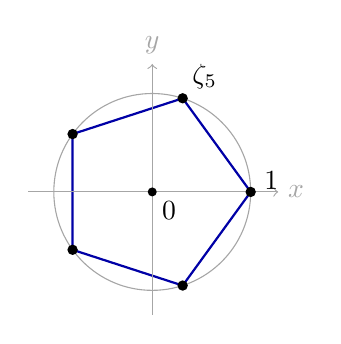
\begin{tikzpicture}[scale=1.25]
  \draw[gray!70] (0,0) circle (1);
  \foreach \j in {0,...,4}{
    \coordinate (P\j) at ({cos(72*\j)},{sin(72*\j)});
  }
  \draw[thick,blue!65!black]
     (P0)--(P1)--(P2)--(P3)--(P4)--cycle;
  \draw[gray!70,->] (-1.26,0)--(1.28,0) node[right] {$x$};
  \draw[gray!70,->] (0,-1.25)--(0,1.3) node[above] {$y$};
  \fill (0,0) circle(1.3pt) node[below right] {$0$};
  \foreach \j in {0,...,4}{\fill (P\j) circle(1.5pt);}
  \node[anchor=west] at (1.04,0.12) {$1$};
  \node[anchor=south west] at (P1) {$\zeta_5$};
\end{tikzpicture}
\end{center}
Rysunek pokazuje jednostkowy okrąg oraz wszystkie pięć
wierzchołków otrzymanych z jednego skonstruowanego punktu
$\zeta_5$. Jest to ilustracja położeń, a nie zastępstwo
dowodu konstruowalności współrzędnych.
\end{przyklad}
